%%
%% This is file `sample-manuscript.tex',
%% generated with the docstrip utility.
%%
%% The original source files were:
%%
%% samples.dtx  (with options: `manuscript')
%% 
%% IMPORTANT NOTICE:
%% 
%% For the copyright see the source file.
%% 
%% Any modified versions of this file must be renamed
%% with new filenames distinct from sample-manuscript.tex.
%% 
%% For distribution of the original source see the terms
%% for copying and modification in the file samples.dtx.
%% 
%% This generated file may be distributed as long as the
%% original source files, as listed above, are part of the
%% same distribution. (The sources need not necessarily be
%% in the same archive or directory.)
%%
%% The first command in your LaTeX source must be the \documentclass command.
%%%% Small single column format, used for CIE, CSUR, DTRAP, JACM, JDIQ, JEA, JERIC, JETC, PACMCGIT, TAAS, TACCESS, TACO, TALG, TALLIP (formerly TALIP), TCPS, TDSCI, TEAC, TECS, TELO, THRI, TIIS, TIOT, TISSEC, TIST, TKDD, TMIS, TOCE, TOCHI, TOCL, TOCS, TOCT, TODAES, TODS, TOIS, TOIT, TOMACS, TOMM (formerly TOMCCAP), TOMPECS, TOMS, TOPC, TOPLAS, TOPS, TOS, TOSEM, TOSN, TQC, TRETS, TSAS, TSC, TSLP, TWEB.
% \documentclass[acmsmall]{acmart}

%%%% Large single column format, used for IMWUT, JOCCH, PACMPL, POMACS, TAP, PACMHCI
% \documentclass[acmlarge,screen]{acmart}

%%%% Large double column format, used for TOG
% \documentclass[acmtog, authorversion]{acmart}

%%%% Generic manuscript mode
\documentclass[acmsmall]{acmart}

%%
%% \BibTeX command to typeset BibTeX logo in the docs
\AtBeginDocument{%
  \providecommand\BibTeX{{%
    \normalfont B\kern-0.5em{\scshape i\kern-0.25em b}\kern-0.8em\TeX}}}

%% Rights management information.  This information is sent to you
%% when you complete the rights form.  These commands have SAMPLE
%% values in them; it is your responsibility as an author to replace
%% the commands and values with those provided to you when you
%% complete the rights form.
\setcopyright{acmcopyright}
\copyrightyear{2020}
\acmYear{2020}
\acmDOI{10.1145/1122445.1122456}

%% These commands are for a PROCEEDINGS abstract or paper.
\acmConference[CSCW '20]{Woodstock '18: ACM Symposium on Neural
  Gaze Detection}{June 03--05, 2018}{Woodstock, NY}
\acmBooktitle{Woodstock '18: ACM Symposium on Neural Gaze Detection,
  June 03--05, 2018, Woodstock, NY}
\acmPrice{15.00}
\acmISBN{978-1-4503-9999-9/18/06}


%%
%% Submission ID.
%% Use this when submitting an article to a sponsored event. You'll
%% receive a unique submission ID from the organizers
%% of the event, and this ID should be used as the parameter to this command.
%%\acmSubmissionID{123-A56-BU3}

%%
%% The majority of ACM publications use numbered citations and
%% references.  The command \citestyle{authoryear} switches to the
%% "author year" style.
%%
%% If you are preparing content for an event
%% sponsored by ACM SIGGRAPH, you must use the "author year" style of
%% citations and references.
%% Uncommenting
%% the next command will enable that style.
%%\citestyle{acmauthoryear}

%%
%% end of the preamble, start of the body of the document source.
\begin{document}

%%
%% The "title" command has an optional parameter,
%% allowing the author to define a "short title" to be used in page headers.
\title{``If there were other options\textellipsis'': 
How Quadratic Voting aligns with people's true preferences.}

%%
%% The "author" command and its associated commands are used to define
%% the authors and their affiliations.
%% Of note is the shared affiliation of the first two authors, and the
%% "authornote" and "authornotemark" commands
%% used to denote shared contribution to the research.
% \author{Author 1}
% \authornote{Both authors contributed equally to this research.}
% \email{email@address.com}
% \author{Author 2}
% \authornotemark[1]
% \email{email@address.com}
% \affiliation{%
%   \institution{Institute for Clarity in Documentation}
% }

% \author{Lars Th{\o}rv{\"a}ld}
% \affiliation{%
%   \institution{The Th{\o}rv{\"a}ld Group}
%   \streetaddress{1 Th{\o}rv{\"a}ld Circle}
%   \city{Hekla}
%   \country{Iceland}}
% \email{larst@affiliation.org}

% \author{Valerie B\'eranger}
% \affiliation{%
%   \institution{Inria Paris-Rocquencourt}
%   \city{Rocquencourt}
%   \country{France}
% }

% \author{Aparna Patel}
% \affiliation{%
%  \institution{Rajiv Gandhi University}
%  \streetaddress{Rono-Hills}
%  \city{Doimukh}
%  \state{Arunachal Pradesh}
%  \country{India}}

% \author{Huifen Chan}
% \affiliation{%
%   \institution{Tsinghua University}
%   \streetaddress{30 Shuangqing Rd}
%   \city{Haidian Qu}
%   \state{Beijing Shi}
%   \country{China}}

% \author{Charles Palmer}
% \affiliation{%
%   \institution{Palmer Research Laboratories}
%   \streetaddress{8600 Datapoint Drive}
%   \city{San Antonio}
%   \state{Texas}
%   \postcode{78229}}
% \email{cpalmer@prl.com}

% \author{John Smith}
% \affiliation{\institution{The Th{\o}rv{\"a}ld Group}}
% \email{jsmith@affiliation.org}


% %%
% %% By default, the full list of authors will be used in the page
% %% headers. Often, this list is too long, and will overlap
% %% other information printed in the page headers. This command allows
% %% the author to define a more concise list
% %% of authors' names for this purpose.
% \renewcommand{\shortauthors}{Trovato and Tobin, et al.}

%%
%% The abstract is a short summary of the work to be presented in the
%% article.
\begin{abstract}
  A clear and well-documented \LaTeX\ document is presented as an
  article formatted for publication by ACM in a conference proceedings
  or journal publication. Based on the ``acmart'' document class, this
  article presents and explains many of the common variations, as well
  as many of the formatting elements an author may use in the
  preparation of the documentation of their work.
\end{abstract}

%%
%% The code below is generated by the tool at http://dl.acm.org/ccs.cfm.
%% Please copy and paste the code instead of the example below.
%%
\begin{CCSXML}
<ccs2012>
 <concept>
  <concept_id>10010520.10010553.10010562</concept_id>
  <concept_desc>Computer systems organization~Embedded systems</concept_desc>
  <concept_significance>500</concept_significance>
 </concept>
 <concept>
  <concept_id>10010520.10010575.10010755</concept_id>
  <concept_desc>Computer systems organization~Redundancy</concept_desc>
  <concept_significance>300</concept_significance>
 </concept>
 <concept>
  <concept_id>10010520.10010553.10010554</concept_id>
  <concept_desc>Computer systems organization~Robotics</concept_desc>
  <concept_significance>100</concept_significance>
 </concept>
 <concept>
  <concept_id>10003033.10003083.10003095</concept_id>
  <concept_desc>Networks~Network reliability</concept_desc>
  <concept_significance>100</concept_significance>
 </concept>
</ccs2012>
\end{CCSXML}

\ccsdesc[500]{Computer systems organization~Embedded systems}
\ccsdesc[300]{Computer systems organization~Redundancy}
\ccsdesc{Computer systems organization~Robotics}
\ccsdesc[100]{Networks~Network reliability}

%%
%% Keywords. The author(s) should pick words that accurately describe
%% the work being presented. Separate the keywords with commas.
\keywords{datasets, neural networks, gaze detection, text tagging}


%%
%% This command processes the author and affiliation and title
%% information and builds the first part of the formatted document.
\maketitle
\section{Introduction}
Decision-makers often utilize surveys to aggregate opinions from the crowd to inform decisions. Understanding a crowd's preferences and priorities across a set of options under resource constraints is a common use case of surveys. \tc{When there are insufficient resources, such as money, time, space, and workforce, it is impossible to satisfy all the needs, creating a resource constraint scenario. Examples of these scenarios include public polling surveys designed to allocate government budgets \cite{pew_spending}, surveys to assess designs in human-computer interaction (HCI) interfaces \cite{ledo2018evaluation}, and surveys to prioritize what products to stock in grocery stores \cite{nielsen}.}

Likert scale is the current norm in many survey settings \cite{moors2016two}, including resource-constrained collective decision-making, because it is easy to administer and understand. For example, the Pew Research Center administered annual surveys with a 3-point Likert-like scale to \tc{know} how participants would budget federal government resources \cite{pew_spending}. In a Likert-like scale survey, participants can freely select ``increase spending'' for all government program areas without considering its feasibility under a limited government budget, a behavior known as the ``extreme responding'' bias \cite{batchelor2016extreme, furnham1986response, meisenberg2008acquiescent}. In this case, the inability to accurately elicit people's true preferences can lead to sub-optimal government budget allocation. Challenges with eliciting accurate self-reported preferences in resource-constrained decisions motivated us to examine an alternative, Quadratic Voting (QV), a relatively new voting mechanism proposed by \textcite{posner2018radical}. In this paper, we empirically tested how well QV elicits true preferences in resource-constrained collective decision-making processes compared to the Likert scale. \lwt{Here, we define an individual's ``true preference'' as a preference based entirely on their honest opinions and their own will.} \tc{We measure it through the outcome of an incentive-compatible task in our study.}

\tc{When making decisions under resource-constrained scenarios}, decision-makers ask the crowd two questions: (a) \textit{how much} do you prefer each option, and (b) how would you prioritize (i.e., rank) the options? Throughout the past century, researchers developed various forms of surveys to elicit true preferences via self-reporting. Ratings and rankings approaches are two of the primary categories in survey methods; they focus on answering one of the two questions above, but not both \cite{moors2016two}. 

% Ratings approaches, such as those used in Likert scales \cite{likert1932technique}, elicit attitude intensity to answer question (a), while ranking approaches that use a ranking scale \cite{starch1923methods}, ask question (b) \cite{moors2016two}. These limitations motivated us to examine an alternative that combines approaches from ratings and rankings, Quadratic Voting (QV), a relatively new voting mechanism proposed by \textcite{posner2018radical}. In this paper, we empirically tested how well QV elicits true preferences in resource-constrained collective decision-making processes compared to the Likert scale, the current norm in these processes \cite{moors2016two}.

% In order to find truthful answers, researchers have developed various forms of surveys to elicit \textit{truthful} self-reported preferences \cite{stone1999science}. 
% Rating and ranking-based surveys are the two major categories \cite{moors2016two}, each with their strengths and weaknesses. 

When responding to opinion-related questions in a rating-based survey, survey takers indicate their level of agreement, satisfaction, or importance along an intensity scale \cite{moors2016two}. The Likert scale is the most commonly used rating-based technique that elicits the \textit{strength} of a survey taker's preferences \cite{likert1932technique}. Rating-based surveys are easy to understand and administer; this may explain why the Likert scale is the current norm in many survey settings. In a resource-constrained scenario, however, a Likert scale survey may not accurately elicit how participants \textit{prioritize} \tc{the options since each option's statement is independent \cite{alwin1985measurement},} and a Likert scale survey does not safeguard against exaggerated or unrealistic preferences \cite{araujo2017much, vavreck2007exaggerated}.

On the contrary, ranking-based surveys focus on understanding how participants \textit{prioritize} the possible options \cite{moors2016two}, naturally incorporating the notion of resource constraints. For example, in participatory budgeting \cite{cabannes2004participatory}, a resource-constrained collective decision-making scenario where citizens vote for the projects that go into a government budget, participants use ranked voting to order the list of projects according to their relative preferences \cite{benade2020preference}. However, ranking-based surveys cannot elicit the \textit{strength} of a participant's preferences, i.e., how much more a participant values option A over B. Besides, performing statistical analysis on rankings data is challenging \cite{alwin1985measurement}.

There had been long debates on the pros and cons of rankings and ratings approaches. Nonetheless, when researchers developed many of these survey methodologies, the mediums of conducting surveys were paper and landlines. The current generation of survey tools, such as Survey Monkey and Qualtrics, simply translated the traditional approaches from paper to online. Given the ubiquity of personal computing devices today, such as \tc{smartphones, tablets,} and laptops, we ask: is there a computational-powered survey methodology that elicits both the rankings \textit{and} ratings of a set of options accurately in a resource-constrained collective decision-making process? In this study, we investigate Quadratic Voting (QV) \cite{posner2018radical} as a potential response to this question. 

Participants rank and rate the potential options in QV at the same time. In QV, expressing an opinion is not free -- each participant receives a fixed budget of voice credits, i.e., the ``currency" in QV, and pays a quadratic cost for the votes they cast. More formally, casting $n$ votes for or against an option costs $n^2$ voice credits. Participants vary the number of votes to represent the strength of their preference, i.e., they \textit{rate} an option with the number of votes. But as the number of votes on an option increases, the marginal cost for each extra vote increases as well; in other words, each additional vote becomes more expensive. Participants may cast as many votes as they choose on any option, as long as the total cost for the votes does not exceed the fixed given budget of voice credits. The limited budget and increasing marginal cost \tc{encourage} participants to make trade-offs among options, equivalent to \textit{ranking} them. Prior work further demonstrated that QV outcomes approximated a normal distribution\tc{ instead of }the polarized responses from Likert scale survey results on highly-debated topics \cite{quarfoot2017quadratic}. However, to the best of our knowledge, no one has empirically explored whether QV \tc{can elicit} more accurate self-reported preferences.
%\textcite{lalley2018quadratic} proved that the QV mechanism is more Pareto-optimal than many traditional voting mechanisms.

In our study, we examined QV's ability to elicit true preferences in resource-constrained collective decision-making processes. Given that Likert scale surveys are the most widely adopted to date \cite{moors2016two}, we compared a QV survey to a Likert scale survey \cite{likert1932technique} in a resource-constrained setting. We identified two distinct types of survey questions in this setting: (1) choosing among $K$ independent options of one topic, and (2) choosing among $K$ dependent options that jointly contribute to the same topic. To offer an analogy, scenario one relates to choosing among ice cream, cakes, and puddings for dessert, while scenario two assesses what an individual cares more about when choosing ice cream -- the flavor, texture, or ingredients. Therefore, we analyzed them in two separate research questions:


\begin{itemize}
    \item[\textbf{RQ 1}] How do QV responses align with people's true preferences compared to Likert scale responses in a survey where survey respondents choose among $K$ independent options of one topic? How do variations in the number of voice credits given to QV survey respondents impact this outcome?

    \item[\textbf{RQ 2}] How do QV responses align with people's true preferences compared to Likert scale responses in a survey where survey respondents choose among $K$ dependent options that jointly contribute to the same topic? 
\end{itemize}

To answer RQ1, we designed a public polling survey to assess which social causes need more support, a typical scenario for choosing among $K$ independent options. To measure participants' true preferences on the same topic, we created an incentive-compatible donation task, in which participants should only donate more for cause A than cause B if they truly care more about cause A \cite{champ1997using}. Participants on Mechanical Turk (MTurk) completed either a 5-point Likert scale version or a QV version of the survey, and the donation task, in a randomized controlled experiment. \tc{Since we were not aware of any prior work that empirically explored a way to determine the voice credit budget of QV, we asked the second question in RQ1. We experimented with} three variations of the QV survey with a small ($O(K)$), medium ($O(K^{1.5})$), and large ($O(K^2)$) budget in the experiment. We measured the similarity between each individual's survey result and their true preferences as reflected in the donation task and applied Bayesian analysis to compare the degree of similarity to true preferences in QV and Likert scale surveys.

In the case of choosing among $K$ dependent options that jointly contribute to the same topic in RQ2, we used an HCI user study scenario to understand how users make trade-offs across visual and audio elements in a video streaming experience given limited internet bandwidth. We used QV and 5-point Likert scale surveys to obtain participants' self-reported responses and designed \tc{an} incentive-compatible product design and pricing task to elicit their willingness-to-pay for each video element \cite{roth1982incentive}. Similar to the first experiment, we conducted the randomized controlled experiment on MTurk and analyzed the results with Bayesian analysis.

\textbf{Contributions} This work contributes to the extensive body of work on survey techniques that elicit self-reported preferences in resource-constrained decision-making in two ways: we find an improved accuracy of responses via QV compared to the Likert scale norm, and we extend the use of QV to the HCI user study domain.

\begin{description}
\item[QV elicits true preferences more accurately:] We show empirically that QV with a medium (i.e., $O(K^{1.5})$) to large (i.e., $O(K^{2})$) voice credit budget elicits true preferences more accurately than Likert scale responses when the survey respondents are asked to either (1) choose among $K$ independent options of the same topic, or (2) choose among $K$ dependent options jointly contributing to the same topic, under resource constraints. \tc{Unlike} prior empirical work that compared the characteristics of QV and Likert scale responses \cite{quarfoot2017quadratic, naylor2017first}, we focus on accurate preference elicitation. Based on two carefully-designed randomized controlled experiments, our Bayesian analysis showed that QV responses aligned significantly closer to participants' responses in an incentive-compatible task \tc{than the} 5-point Likert scale responses with a medium to high effect size. This finding is important because it shows that QV, a computational-powered alternative survey approach that combines ratings and rankings, \tc{can} assist resource-constrained decision-making with more accurate self-reported responses.
\item[Application of QV to HCI:] We extend QV's application scenario from typical public policy and education research to a problem setting familiar to the CSCW community: a prototypical HCI user study. The limited empirical studies and applications of QV focused mostly on public policy \cite{quarfoot2017quadratic, colorado_qv} and education research \cite{naylor2017first}. To the best of our knowledge, no HCI study has applied QV in a survey before. We designed an HCI user study with a research question that involved resource-constrained decisions and showed that a QV survey \tc{could} elicit users' preferences on an HCI-related research question more accurately than a Likert scale survey, a norm in the HCI community \cite{ledo2018evaluation}. Our experiment results, QV survey design, and QV interface serve as a stepping stone for HCI researchers to further explore the use of this surveying method in their studies and encourage decision-makers from other fields to consider QV as a promising alternative.
\end{description}

While our study demonstrates the potential of QV as a computational tool to facilitate truthful preference elicitation, the goal of this research is \textit{not} to convince decision-makers to replace their Likert scale surveys with QV surveys entirely. Indeed, in cases including when the survey requires the use of \tc{paper-based} responses (e.g., when technological aids are unavailable) or when the survey involves a list of unrelated options, QV may not be an appropriate option. Instead, our goal with this paper is to show that in the ratings and rankings scenarios that we investigate in this paper, QV may prove to be a compelling alternative to \tc{the} Likert scale when conducting online surveys.  

% we pose many open questions to prompt further conversations in the community, and encourage decision-makers to carefully evaluate QV's strengths and weaknesses (e.g., higher cognitive cost, less known to participants) prior to adoption.
% accuracy


% wider application domains



% ask participants to express their attitudes using a scale for a given topic or question on a scale of 1 to 5. Researchers would use collected responses to make their decision. This paper focuses on collective decision-making tasks aimed at eliciting group preferences among a set of choices among $K$ options. Questions such as: ``Which interface do users like most?'', ``What are some products that customers are satisfied with?'', and  ``What public policies do constituents feel more important?'' are examples of eliciting group preferences among $K$ options.


% \textit{RQ1.} How do results from QV, Likert survey align with people's incentive-compatible behavior when surveying societal issues? 

% We designed an experiment to compare how participants donate with QV and Likert survey results. We analyzed data using Bayesian analysis and qualitative analysis. We hypothesized that QV results better portray individuals' true beliefs as reflected by their monetary donations.

% \textit{RQ2.} How do results from QV and Likert-scale align with people's incentive-compatible behavior with a choice of HCI research questions? 
% To the best of our knowledge, no HCI studies used QV in their studies. Similar to the first experiment, we compare results from QV and Likert surveys with participant's behaviors in a video-element HCI experiment. We hypothesize that QV more accurately reflects the intensity of individuals' true beliefs. 

% \textit{RQ3.} How do different quantities of voice credits impact the results of QV empirically?
% We did not find studies on how many voice credits a participant should receive for QV in related literature. In conjunction with RQ1, we provide participants with a different number of voice credits. We suspect different outcomes from QV when participants have a different number of voice credits.


% is prone to reduced data quality. 
% Since each statement of Likert survey is independent when answering, \textcite{alwin1985measurement} found participants respond with the first acceptable answer instead of compiling an optimal solution. Another fallacy follows similar logic where participants would express opinions to the extreme, exaggerating one's actual belief \cite{araujo2017much, vavreck2007exaggerated}. This is due to Likert survey's nature of not incorporating the notion of resource constraints in the real word where it actually exists, for example, in the case of allocating budget for government spending. Participants in the example could express having large budgets for all causes, which in reality, in not possible because the budget is limited. Some researchers tried to introduce constraints to rating based surveys, for instance knapsack voting, developed by \textcite{goel2015knapsack}, forces participants to elect agreement only if the sum of the cost for the selected items is less than a given budget.

% For example, ranking scales is a ranking-based technique created by \textcite{starch1923methods} in 1923. Participants ranks a list of options in the order of their preferences in a ranking scale survey. Though researchers believe ranking demonstrated better reflects individuals' accordance, they are harder to statistically analysis and more cognitive demanding to participants \cite{moors2016two}. In other words, people are forced to make distinctions between options for rank-based surveys and applying constraints, i.e., there can only be one item ranked first. When taking budget into considerations, researchers developed value-for-money-ranking which asks participants to rank according to not just how they value the options, but the value-cost ration of the options. The biggest drawback of rank-based methods is giving up the information of \textit{strength} among their standings, i.e., how far apart is the first preference compared with the second? 


% Since early 1980s when investigators start to distribute surveys using internet-connected devices, electronic-mediated surveys merely translate paper-based surveys onto a webpage. Researchers did not make noticeable changes on the \textit{survey mechanisms} that unleashes the power of computation. Given the computing power of computers today and the omnipresence of computers at any individual's hands, can a better surveying mechanism harness computational advantages to obtain more accurate survey results?

% In this paper, we examine an alternative, Quadratic Voting (QV), a relatively new voting mechanism proposed by \textcite{posner2018radical}, to elicit more truthful self-reported responses in resource-constrained collective decision making processes. 

% Distribution of surveys for resource-constrained decision making is pervasive in everyday life and these surveys have been effective at aggregating people's attitudes to form consensus. Think tanks design and deploy large-scale ordinal scale polls \cite{pew} to understand public opinions on government policies given limited government resources. Supermarkets collect individuals' shopping experiences across products because there are limited shelves \cite{nielsen}. 

%% electronic decision making surveys merely transform from paper, but hasn't done much extra with the computational power; 
% Before the 1980s, research surveys required large-scale in-person participation. Slowly, surveys evolved into mail-in, telephone, and, eventually, online formats. In the early 1980s, researchers introduced electronic surveys to individuals as internet-connected devices became accessible. \kk{How did people take these? Not too many people had ISP service in the 80s. Which companies administered them?} They are limited to international companies and fortune 500 in 1985. Electronic surveys aimed to reduce research costs, reduce human labor required to conducted surveys, and add additional flexibility in survey design\cite{kiesler1986response}. While the \textit{medium} of how researchers conducted the surveys moved from offline to online, researchers did not make noticeable changes on the \textit{survey mechanisms} that unleashes the power of computation. We argue that electronic-mediated surveys merely translate paper-based surveys onto a webpage. Given the computing power of computers today and the omnipresence of computers at any individual's hands, can a better surveying mechanism harness computational advantages to obtain more accurate survey results?

% QV is an example of utilizing the computational power, and have xxx, xxx, xxx proven benefits in previous work; 

% In this study, , given that quadratic computations are difficult to conduct on paper or verbally due to the required cognitive load.

% we also want to confirm if QV is "accurate" enough in soliciting people's opinions
% Since Likert is the most commonly used form of a survey; we compare QV's accuracy with Likert's; 
% Since surveys are deployed to accurately understand people's attitudes, this paper aims to understand how how well QV survey results align with real world behaviors and beliefs?. To the best of our knowledge, there have not been any empirical studies that investigated to what degree does QV results align with participants' underlying true preferences. 


%Self reported data, that is data supplied by the survey participant is at the core of such surveys across a wide range of disciplines, from medicine to social services \cite{stone1999science}. To address this, researchers, have designed different types of survey mechanisms throughout the past century. In 1923, 
%In another survey approach, pairwise preference, developed by \textcite{scheffe1952analysis} in 1952, participants compared two choices by stating their preferences in one of seven intensity levels. Researchers developed these methods to better elicit individual attitudes under different settings and for different goals. Many of the proposed methods, however, fail in capturing authentic signals due to self-reporting bias or <define it>.
% how to use a survey and when to use it is also important
%

% This paper offers three major contributions.
% First, we designed two empirical studies and found that QV aligns better with the participant's underlying preferences when surveying people's preferences among $K$ options. The first experiment looked at eliciting societal causes while the other experiment pertains to HCI. Both of these experiments used participant behaviors as a baseline to measure these differences, which we argue is much stronger than the direct comparison to Likert that prior studies lean on. The results allowed us to argue that researchers should harness computers' power to utilize and benefit from deploying QV in studies if the study aims to understand people's preferences among $K$ options.

% Second, we demonstrate that QV results depend on the voice credit budget. To the best of our knowledge, little did researchers discussed the effect of the number of voice credits in prior works. In this study, we discovered that participants need a large enough voice credit to obtain an accurate QV result.

% The third contribution demonstrates the application of QV in the HCI domain. We are not aware of prior studies in HCI that utilize QV, and we believe that our experiment and software deliverable provides a template to use QV in later research.












%%----------------------------%%




% understanding how to apply QV in real-world scenarios, what challenges QV might face, and design decisions that can influence QV participants.

% \textbf{Design Implication}
% TODO. Talk about interface, future work and insights.


% Our first question focused on whether QV consistently produces a different result from the Likert survey results in an HCI study. Although usually applied to surveys in the social sciences, we hypothesize that QV could produce a cleaner and more accurate result than a Likert survey in an alternative setting such as Human-Computer Interaction (HCI). We designed one pretest experiment and one follow-up experiment to verify our hypothesis. In the pretest, we replicated the study developed by Quarfoot et al. \cite{quarfoot2017quadratic} and swapped the content of the survey with an HCI security study by Leon et al. \cite{leon2013matters} to show that QV extracts more fine-grain information compared to Likert. Results from the pretest aligned with the results by Quarfoot et al., suggesting that QV works under scenarios outside of societal-focused settings. 

%%%%%%%% old text from thesis
% Commercial companies deploy online surveys to understand which improvements users would like to see prioritized for a similar constraint. 
% Other surveys can be found in shopping centers to . 
% Data scientists and product teams also use surveys for them to prioritize mission-critical issues that customers face when deploying a product upgrade. 
% All these examples demonstrate how prevalent groups and institutions used surveys to make decisions by gathering consensus from surveying individual's attitudes.
% Our second question regards how QV and Likert-scale align with an individual's preferences expressed via their behavior across societal issues. We carefully redesigned a new experiment involving a larger group of participants to compare the alignment of QV and Likert surveys with a person's actual behavior. In this experiment, participants expressed their attitudes across societal causes and were given the option to donate to charitable organizations associated with each cause. We took a Bayesian approach to analyze the statistical power and effect size of how closely the Likert Survey and QV align with one's donation distribution. The results found statistical evidence that QV outperforms Likert if there are enough voice credits. Our third question looked at whether a different number of voice credit budget impacts people's voting behavior in QV. We used both experiments, the pretest experiment, and the formal experiment to test this idea. We found through qualitative and quantitative analysis that QV surveys require a significant amount of voice credits. We describe these research question more thoroughly in Chapter \ref{RQ}.

% Since then, this surveying method has been fully adopted by researchers and marketers alike. 
% Some researchers attributed this to the survey's ease of use. However, this ease of use does not guarantee the ease of analysis. Researchers today easily misuse Likert surveys by applying the incorrect analysis methods \cite{bishop2015use} or misinterpreting the analysis results \cite{jamieson2004likert, pell2005use}, leading to doubtful findings. Examples of such includes calculating the mean and standard deviations to interpret the data collected through a Likert survey. Even when applied correctly, there is usually little justification for using Likert surveys over other research tools in their research. 

% and how well it aligns with other surveying methods such as Likert survey. Further, we did not find any empirical study examining whether a different amount of voice credits impacts QV's result.
% Researchers have compared the Likert survey with QV from empirical and theoretical perspectives \cite{quarfoot2017quadratic, naylor2017first}. Cavaille et al. argued that QV outperforms Likert surveys among a set of political and economic issues \cite{cavaille2018towards}. 

% Surveys have been a useful tool at aggregating 
% Research agencies, industry labs, or independent researchers often hope to understand how to allocate resources better or to address people's preferences more accurately. 
% Agencies collect these surveys of huge crowds as a form of collective decision making. 


%%%%%%% old text from QV draft
% Likert survey is one of the most widely used methods to obtain the participant's opinion in the realm of human-computer interaction. Survey participants would express a rating across a series of measurements --- \textit{Very agree to very disagree} or \textit{On a scale of 1 to 5} --- for a listed statement. Very often, these opinions help researchers or decision-makers uncover consensus  across a group of people. However, there had been findings of how researchers can easily misuse Likert surveys either applying incorrect analysis methods  \cite{bishop2015use} or misinterpreting the analysis results \cite{jamieson2004likert, pell2005use} leading to questionable findings.In addition,  many research papers do not explain the rational behind the use of  Likert surveys. In a community that adopted Likert surveys almost as the defacto standard, we ask a fundamental question: ``Is Likert-scale survey the ideal method to measure collective attitudes for decision making?''
% Research agencies, industry labs or independent researchers often want to understand how to better allocate resources or what to improve upon. This is an example of eliciting user preferences  among $K$ options. These opinions are collected among huge crowds, as a form of collective decision making. For example,  ordinal scale polls were designed to understand public opinions on government policy \cite{pew} because there is limited funding. Companies deploy online surveys  to understand how product users  feel about the features and services that needs further improvements because companies have limited time  to develop the next release. Physical surveys can be found  in shopping centers to collect an individual's experiences for products on the shelf because there are limited shelves. All these examples demonstrated how surveys are often tied to  making decisions  by gathering consensus from surveying individual's attitudes. 
% In this study, we look at an alternative method called Quadratic Voting (QV). Published in 2015, \textcite{posner2018radical} proposed Quadratic voting as a voting mechanism with approximate Pareto efficiency.Under this voting mechanism,voters were initially given a fixed amount of voice credits (VC).With the credits, individuals can purchase any number of votes to support any of the statementslisted on the ballot. However, the cost of each vote increases quadratically when voted toward the same option.The authors proved that this mechanism is more efficient at making a collective decision because it minimizes welfare loss.Since 2015, a few studiescompared Likert surveys with QV empirically and theoretically\cite{quarfoot2017quadratic, naylor2017first}.\textcite{cavaille2018towards} argues that QV reflects one's opinion better compared to Likert-scale surveys when surveying one's opinionamong a set of political and economic issues.Despite these findings,we are not aware of related works thatcompare Likert surveys and QVwith participants' underlying true preferences.Therefore, it is unclear whether or notand in what degreedoes QV results align with participants' behaviors.In addition, no current work, to the best of our knowledge,deployed QV in the area of HCI.
%\end{enumerate}
% To answer these research questions,
% we designed two experiments.
% The first experiment,
% designed to answer RQ1 and RQ3,
% is a between-subject study
% where participants express their attitudes
% among a set of societal causes using 
% QV and Likert surveys
% and then donate
% to organizations relevant to these organizations.
% The second experiment 
% created an HCI study environment,
% aimed to answer RQ2,
% where participants were asked about 
% opinions among different video elements
% and their opinions using QV and Likert surveys.
% Our results showed that both experiments support
% QV in providing a clean and efficient way
% compared to Likert surveys
% at eliciting participant's true preferences.

\section{Related Works} \label{related_works}
In this section, 
we present related works
that discussed the challenges
of Likert survey
and related works of QV.

\subsection{Likert Scale Surveys}
Likert surveys are commonly deployed
to collects participant's opinions
because of its ease of use.
These surveys are deployed
to validate findings or clarify hypotheses
\cite{ozok2009survey, ledo2018evaluation} in HCI.
They are also used to verify or uncover the user's needs.
Likert surveys were invented by \textcite{likert1932technique} 
in \citeyear{likert1932technique},
which utilized a scale to deploy step-intervals 
from one attitude to the next.
Researchers today design 3, 5, 7, 
or even 12-point Likert surveys to accommodate different uses
\cite{garland2008computer,finstad2010}.
In addition, these surveys
can ause verbal descriptions
to segment the intervals,
presenting the choices with an ordinal scale.
Some researchers looked at
alternative presentations of the Likert scale
such as slider scales \cite{roster2015exploring} 
or phrase completions \cite{hodge2003phrase}, 
which aimed to circumvent 
some of the shortcomings of the traditional Likert scale.

There are, however, widespread controversies in the community on
when, why, and how to use Likert surveys \cite{bishop2015use}.
For instance, 
researchers sometimes misuse statistical method,
such as using mean and standard deviations \cite{jamieson2004likert},
to understand outcomes
when working with an ordinal metric.
Quantifying aggregated ordinal scale Likert surveys,
such as an average of ``1.5 agree'' can be unclear,
given that there does not exist ``agree and a half''
in real life.
Besides, 
options on the Likert scale can be stepwised.
One should not assume scale intervals to be equal.
In other words,
the difference between
``strongly agree'' and ``agree'' can be different 
when compared to the difference between
``neutral'' and ``agree'' \cite{jamieson2004likert, edmondson2005likert}.

An empirical study by \textcite{quarfoot2017quadratic}
identified another challenge
where people exaggerate their views
when filling out political surveys.
In this study,
participants often express polarized opinions
or have no opinion at all,
making it hard to form optimal conclusions \cite{posner2018radical}.
% When the results were aggregated, 
% a ``W'' shape distribution.
%This distribution demonstrated how people stand upon polarized views,
This occurrence was 
theoretically proved by \textcite{cavaille2018towards},
where respondents tend to overstate their values
if they want to influence the results through the survey.
These challenges motivated us 
to understand whether QV can fill the gap of inaccuracy
and provide a more accurate measurement
for collective decision making.\par

\subsection{Quadratic Voting}
Voting is often excercised
for collective decision making.
Quadratic voting originated 
from the argument
that current one-person-one-vote (1p1v) system
can easily bias toward the majority's opinion
and omitting the minority's votes.
This phenomenon is termed as 
the ``Tyranny of the Majority''
which criticizes that democratic decision
can easilty neglect those in need 
\cite{posner2018radical}.
In addition, 1p1v suffers the inability
for individuals to express fine-grain opinions
on the options one voted \cite{sep-voting-methods}.
Ranked-based voting tried to resolve this
by allowing voters to rank the options.
This mechanism can
suffer from Condorcet's paradox 
where results can be suboptimal 
because the ranks of the voters
might not be transitive\cite{easley2012networks, sep-voting-methods}.

This motivated the development of Quadratic Voting
created by \textcite{posner2018radical}. 
to overcome traditional voting challenges .
QV captures the cost a voter has to pay
when they made a particular voting decision.
It regulates the votes by assigning different level of prices
given a fix budget.
This "price-taking" equilibrium helps
participants vote by maximizing their utility.
This is theoretically supported by \textcite{lalley2018quadratic}
and showed that there exists an approximate structure of Bayes-Nash equilibria.

In order for QV to capture the voice of the minority
and allocate the correct cost to the votes,
QV established the following mechanism:
Consider collecting votes from $N$ participants,
each participant is entitled to 
$K$ voice credits.
Participants can express binary opinion (for or against)
each option $o_i$ acorss a set of options $O$ listed on the ballot. 
Participants can purchase any number of votes $v_i \in \mathbb{R}$
vetted toward any of the options $o_i$.
However, to vote $v_i$ votes toward $o_i$,
participants have to spend $v_i^2$ voice credits,
billed toward their $k$ credits.
The outcome of QV 
would be the ranks of the sum
among the total votes for any option $\sum{V_{oi}}$
across all $N$ participants.

To use an analogy,
suppose every voter has a bank account 
with a fixed amount of money, say 100 dollars.
On a ballot, there are ten statements.
Voters can now buy votes using their money in the account.
However, for each statement, the cost of the votes
increases quadratically. 
For example, voting two fors on the first statement 
would cost the voter four dollars;
voting three against on another statement 
costs the voter nine dollars, and so on.
This means that the more votes one devote to an option,
the more costly it is.
Voting more votes on one statment, 
forgoes the opportunity to vote for other options.
Here, the money referes to the voice credit in QV.

\subsection{QV in the wild}
After proposing QV,
\textcite{quarfoot2017quadratic} conducted an 
empirical study to understand how 
QV results compare to Likert scale surveys.
They surveyed 4500 participants 
on individuals' opinions
across ten public policy
using either a Likert survey, QV, or both.
The study found that the number of people
who voted for the same number of votes
for any particular option 
follows a normal distribution when using QV.
This differ from the Likert surveys,
which among the same group of participants,
returned heavily skewed 
or polarized ``W-shaped'' distributions.
Researchers inferred 
QV provides is better at expressing the participant's opinion
for polarized statements.
Researchers also saw individuals 
spent more time expressing their opinion
and reveal a more fine-grain attitude 
toward the policies.
Thus, the study concludes that 
QV provides a clearer picture 
of public opinion to policymakers
\cite{quarfoot2017quadratic}.

The work by \textcite{quarfoot2017quadratic}, however,
only used mean and z-scores,
to compare the final aggregated results 
across the two methods.
In addition, 
the design on the policies 
have a strong tendency for voters
to agree or disagree on the extreme,
such asking one's opinion on ``same-sex marriage''.
Thus, little do we know if
QV produces different results 
than Likert scale surveys
if the options are less competitive,
for example, choosing one's favorite ice cream flavor.\par
% For example, if we are looking at 
% preference elicitation where the group aims to choose
% one among $K$ options.

Another empirical study was applied to 
the field of education 
by \textcite{naylor2017first}. 
The author used QV and Likert survey
to understand essential elements 
among a list of factor
that impacts students' success in universities.
Results showed that QV provided more insights, 
such as distinguishing good-to-have factors from must-have elements.
These factors are not heated debated controversies
compared to public policies in the previous studies, 
but each of the elements are independent and does not require 
students to make trade-offs.
For example, students can have a sense of ``belonging'' and
a sense of ``achievement'' at the same time.

To the best of our knowledge,
there does not exist an empirical study 
that focused on investigating
how QV and Likert perform
under the condition of selecting
one in $K$ options.
% Do note that these trade-offs need not be polarizing topics
% but rather where each option is interconnected
% and can impact one from the other.
This setting was recently discussed 
in a theoretical work by \textcite{eguia2019quadratic}
who claims that QV is still in favor 
of resolving budget-constrained 
for risk natural agents
to figure out an efficient decision 
across multiple alternatives
as a collective choice problem.
We aim to complete this missing piece of the puzzle 
through an emprical study.
Further,
we are not aware of any work
that studies alignment between
participants' actual beliefs
and QV surveys.
Existing research pointed out 
possible fallacy exists with self-reporting
\cite{araujo2017much, vavreck2007exaggerated}.
Thus, we aim to understand
how QV and Likert scale surveys
aligned with the agent's true beliefs
instead of simply comparing 
the outcomes of Likert surveys with QV.
We also want to test
whether the total number of voice credits 
impacted the results of QV.
Finally, we believe that
no HCI research utilized QV
to form design decisions.
\section{Methods}
We designed two experiments to investigate our research questions.
The first experiment applied both QV and Likert-scaled surveys to 
measure people's preferences among societal issues.
We then deployed a donation task to match the results of the surveys to people's preference. 
The second experiment extends upon the first one with a focus
in the context of HCI survey.\par

\subsection{Demographics}

\subsection{Experiment 1}
%Motivation
The first experiment aims to answer the first research question. 
We try to understand how QV aligns with people's true preference
compared to Likert-scaled surveys 
when a group of people is selecting $n$ items among $k$ options.
This experiment also aims to answer the third research question:  
trying to observe if and how different numbers of voice credit 
impact participants QV responses.
Conducted between subjects, 
the first experiment is made up of three primary segment: 
demographics, surveys and donation. This process is demonstrated in graph X(a).\par

%Grouping
Both group of participants will fill out a demographic survey
after agreeing the consent form.
This demographic survey captures participant's basic information 
such as age, gender, income, ethnicity, profession and so on. 
Participants are divided into two groups: QV group and Likert group.
Participants in the QV group 
will first go through a tutorial on what QV is 
and how QV works using a pre-recorded video. 
To make sure that the participants understand the concepts correctly,
they have to correctly answer questions regarding the concepts
in order to move on. 
They would experience 4 QV surveys shown as graphic X(b).\par

%QV
The first two QV surveys asked participants to vote with QV among 9 different societal causes 
based on the causes they think requires more resource allocation. 
The only difference between the first two surveys 
are the number of voice credits the participants have to express their votes. 
The two number of credits a participants can have are equally drawn from 
two of the three possible number of credits: $36$, $108$ and $324$. 
[Explain the three voice credits here] 
The last two surveys are designed to look similar to the first two.
They differ at the set of nine societal causes presented to the participants.
These nine causes have no direct purpose to the experiment. 
They are designed to distract the participants and 
prevent them making connections to the donation task which follows.
Note that the selection of voice credits 
for the first two QV survey 
would be the same for the latter two QV survey. 
The second group of participants 
completes two Likert-scaled surveys.
The two surveys mirror the nine societal causes 
listed on the first and third QV surveys.
Both surveys are provided in the supplementary materials.\par

%Donation
A donation task is deployed to the participants after the surveys were completed
to measure the true preferences based on participant's behaviors.
Participants are told that for every 70 participants, one participant would win 35 US dollars.
Assuming winning the 35 US dollars, 
the participants were asked if they would want to donate 
some money to some of the nine charity groups.
These nine charity groups mirrors the nine societal causes 
listed on the first two QV survey and the first likert-scaled survey.
Participants are aware that 
the research team will match one dollar to each one dollar they donated to an organization. 
Participants are also aware that 
they get to keep the amount of money not donated to any organizations if winning the lottery.\par

\subsubsection{Selection of the societal causes}


\subsubsection{System Architecture and Interface}
The voting system is constructed using Python Flask for the back-end, 
Angular for front-end and 
MongoDB for database storage. 
The experiment source code is publicly available \footnote{Not yet public} 
and the QV interface is also provided as a stand-alone repository \footnote{https://github.com/hank0982/QV-app}.
In this subsection,
we focus on the QV interface.\par

The QV interface, 
shown in graph Y, 
consists of three major sections.
The first section contains definitions of QV and the prompt of the task.
The second section shows a list of option with a plus and minus button to its left.
Buttons are disabled if the number of voice credit does not permit the next vote.
A bar on the right of the option shows the proportion of voice credits used to that option.
The final section is a floating summary at sticks to the bottom of the page.
It contains a visualization of the total number of credits and the remaining credits.\par

\subsection{Experiment 2}
The second experiment extends upon the first one,
in which it examines 
whether Quadratic Voting betters at aligning people's actual preferences
compared to a Likert-scaled survey in an HCI setting.
Different from political and public-opinion surveys, 
testing participants' preference 
in interface design and user experience 
is much more non-trivial.
Thus we developed a buy-back mechanism 
and observe participants' behaviors 
as their true preference.
This experiment also acts as a concrete example as to how QV can be incorporated in HCI.

\subsubsection{Choice of HCI Research Question}
Research on video and audio quality 
from the lens of HCI 
has been a relatively mature.
Contributions has been made to fields like
multi-media conferencing \cite{watson1996evaluating}, video-audio perception \cite{chen2006cognitive, molnar2015assessing}
and more specifically trade-offs between video and audio elements under network monetary constraints \cite{molnar2013comedy, oeldorf2012bad}.
%These elements can includeing video frame rate, video bit rate, video resolution, video package loss rate, audio package loss rate, audio sampling rate, audio bit rate, audio bit depth, video-audio synchronization, etc. 

Oeldorf-Hirsch et al. \cite{oeldorf2012bad} conducted a study, 
covering the widest range of elements to the best of our knowledge,
to understand how users with bandwidth constraints 
made trade-offs between video and audio elements. 
They examined participants' attitude between three video bit rates, 
three video frame rates and two audio sampling rates 
across three types of video content.
Participants were asked to rate the overall quality, 
video quality, audio quality and enjoyment level 
on a 5-point Likert scale in each condition. 
Conclusion were drawn using mean and standard deviation of the survey results.
This is a typical study 
where the goal is to find  
$1$ or some of the $K$ elements to choose from
when under constraint.
In our second experiment, we expand this study
to collect people's preference among a wider range of video and audio elements 
and compare how Likert-scaled survey and QV reflects people's true perception preferences. 

\subsubsection{Experiment 2 Design}
In our experiment, we included a total of five video and audio element that will impact a video.
These elements include video and audio package loss rate, 
determining whether the audio or video stutters; 
video resolution and audio sampling rate 
effecting the quality of video and audio; 
and video-audio synchronization. 
We selected a few segment of weather broadcasting 
from a news channel 
as the content of our video.
Weather broadcasts usually convey information via both visual and audio channels, 
appeal to a wide array of audiences, 
and do not require prior knowledge to understand.\par

To ensure the ecological validity of the experiment, 
we situated the comparison of different video and audio elements 
in a hypothetical scenario in which the participant 
is a manager of a weather reporting news station. 
As the manager, 
the participant was asked to rate 
the importance of each video and audio elements 
with the goal to maximize customer understanding of the context
where network is of low bandwidth and that the weather broadcast 
cannot be shown in its best quality.\par

We designed a between-subject study
with three groups of 60 participants.
After the participants agreed with the consent form, 
all three group of participant
were presented an example weather broadcast segment
with controls of the five video and audio elements 
under the video shown in figure M. 
All five elements were set to sub-optimal by default, 
making the content near incomprehensible.
Participants can alternate the five elements 
in any combination, 
to see how elements impact to the video.

Once participants think that they had a grasp of 
how different elements impact a video, 
the first group of participants 
then completed a 5-point Likert-scaled survey 
while the second group of participants 
completed a QV survey with K voice credits \footnote{K is decided from experiment 1}, 
asking their opinions 
on the importance of the 5 video and audio elements 
in a weather broadcast 
under a low bandwidth environment. 
The third group of participants 
were asked to perform a buy-back task 
for a bad-quality advertising video.\par

The buy-back task mimics a rational customer's behavior: 
buying essential tools to complete some given task.
Participants were told that 
as the manager of the weather broadcast agency,
they need to verify if their viewer 
can understand the content of the video.
Therefore, the goal of their task 
is to correctly answer a set of multiple choice questions
to make sure that they correctly comprehend the video.
Given the video with sub-optimal video, 
participants were given a budget of \$30 
to purchase some or all of the features back.
To ensure incentive-compatibility 
of the participants' buy-back actions, 
we offered to pay the participants their own remaining amount 
from the \$30 budget through a lottery 
under the condition that 
they answered 80\% of the multiple choice questions correctly,
[missing probability]
version of a new weather broadcast video 
adjusted by their buy-back choices. 
These questions contained factual questions such as, 
"What is the weather of Chicago?", 
"What is the highs and lows of San Diego", 
"Which of the follow cities got colder?". 
Participants were shown three example questions 
before the buy-back task to assist their decision.
Participants can replay the video with their adjustments
while answering the questions
to ensure that participants do not require memorization.
There will be a 5 minute timer to minimize the impact of replaying the video.
With this design, 
participants would try their best to make the video comprehensible 
based on their opinions on which feature(s) was most needed 
at the lowest cost.\par

In the given weather broadcast video, 
there were 4 levels of quality for each of the 5 elements. 
By default, the video set to the lowest level 
for all elements before any adjustment occurred. 
%Based on prior study on the perception of the degradation of the 5 features, we designed the 4 levels to be as linear to user's perception as possible. Below are the 4 levels of the 5 elements listed from the worst to the best quality.

\begin{enumerate}
    \item Audio Package Loss Repaired with Silence (package loss rate) \cite{watson1996evaluating}: 20\%, 10\%, 5\%, 0\%
    \item Video Package Loss (package loss rate) \cite{claypool1999effects}: 20\%, 8\%, 4\%, 0\% (20, 8.3, 3.3, 0) 
    \item Audio Sampling Rate \cite{oeldorf2012bad, noll1993wideband}: 8kHz, 11kHz, 16kHz, 48kHz
    \item Video Resolution \cite{oeldorf2012bad, knoche2008low}: 120x90, 168x126, 208x156, 240x180
    \item Video-audio Synchronization (time video behind audio) \cite{steinmetz1996human}: 240ms, 200ms, 160ms, 0ms (new: 1850, 1615, 1050, 0)
\end{enumerate}

In the buy-back task, 
each level of improvement for one feature costs \$2. 
It would cost the entire budget of \$30 
to buy all levels of every feature back. 
Hence, the option of buying back everything was given to the participants,
in return, there would be no extra payoff remaining for the participant.\par

Similar to the first experiment, 
the money spent on each feature during the buy-back task 
are considered as the true preference 
the population had towards the 5 video and audio features. 
The results from the Likert-scaled surveys and QV survey 
were then compared to the population's true preference 
to see how different they were.\par
\section{Experiment 1 Results} \label{results-1}
\subsection{Experiment 1}



%\begin{acks}
Acknowledgments section
\end{acks}


\bibliography{reference}
\bibliographystyle{ACM-Reference-Format}


%\appendix

\section{Experiment 1 Results}

\subsection{Quantitative Results}
\begin{figure}[htpb]
    \centering
    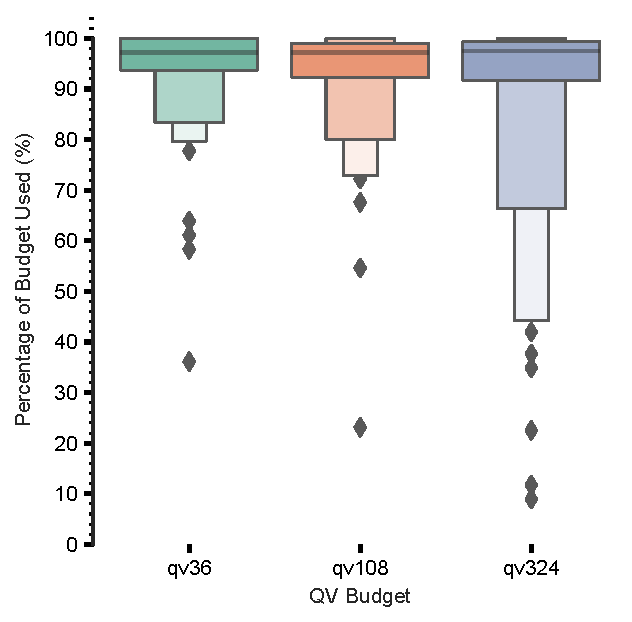
\includegraphics[width=0.5\textwidth, keepaspectratio=true]{content/image/qv_budget_used_distribution.pdf}
    \caption{
      Distribution of Percentage Budget Used in QV36, QV108 and QV324. Percentage budget used is the percentage of voice credits used out of the total voice credits budget available.
    }
    \Description[Distribution of Percentage Budget Used for experiment 1]{Distribution of Percentage Budget Used for experiment 1}
    \label{fig:qv_budget_exp1}
\end{figure}

\subsection{Part Two}

Etiam commodo feugiat nisl pulvinar pellentesque. Etiam auctor sodales
ligula, non varius nibh pulvinar semper. Suspendisse nec lectus non
ipsum convallis congue hendrerit vitae sapien. Donec at laoreet
eros. Vivamus non purus placerat, scelerisque diam eu, cursus
ante. Etiam aliquam tortor auctor efficitur mattis.

\section{Online Resources}

Nam id fermentum dui. Suspendisse sagittis tortor a nulla mollis, in
pulvinar ex pretium. Sed interdum orci quis metus euismod, et sagittis
enim maximus. Vestibulum gravida massa ut felis suscipit
congue. Quisque mattis elit a risus ultrices commodo venenatis eget
dui. Etiam sagittis eleifend elementum.

Nam interdum magna at lectus dignissim, ac dignissim lorem
rhoncus. Maecenas eu arcu ac neque placerat aliquam. Nunc pulvinar
massa et mattis lacinia.

\end{document}
\endinput

